\section{Alvan Alvanzah (1174077)}
\subsection{Tugas Membuat Shapefile dengan PySHP}
\begin{enumerate}
	\item No 1
	\lstinputlisting{src/tugas2/1174077/no1.py}
	\begin{figure}[!htbp]
		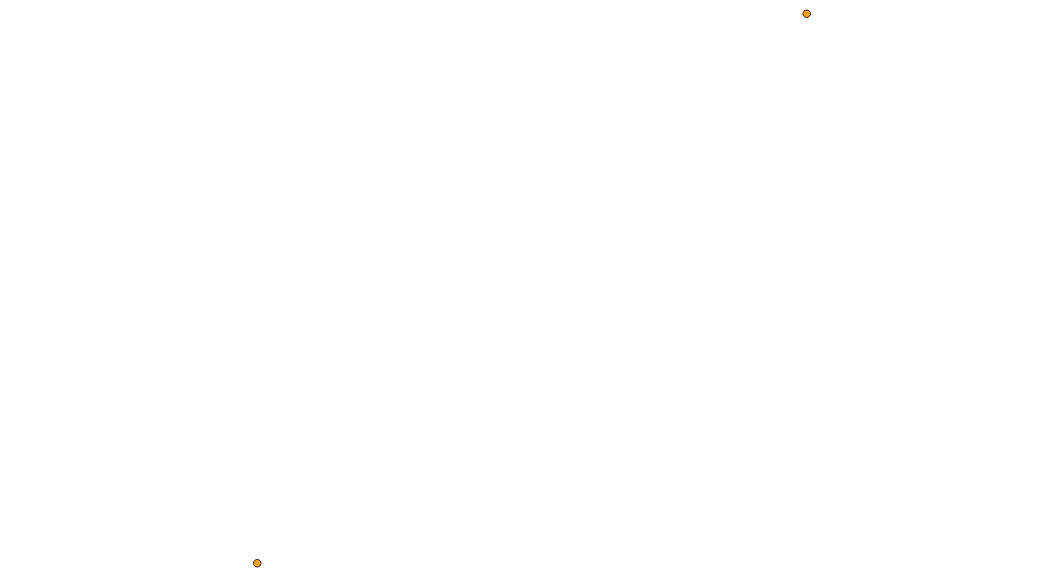
\includegraphics[width=6cm]{figures/Tugas2/1174077/no1.png}
		\centering
		\caption{Hasil No 1}
	\end{figure}
	\item Nomor 2
	\lstinputlisting{src/tugas2/1174077/no2.py}
	\begin{figure}[!htbp]
		
\includegraphics[width=6cm]{figures/Tugas2/1174077/no2.png}
		\centering
		\caption{Hasil No 2}
	\end{figure}
	\item Nomor 3
	\lstinputlisting{src/tugas2/1174077/no3.py}
	\begin{figure}[!htbp]
		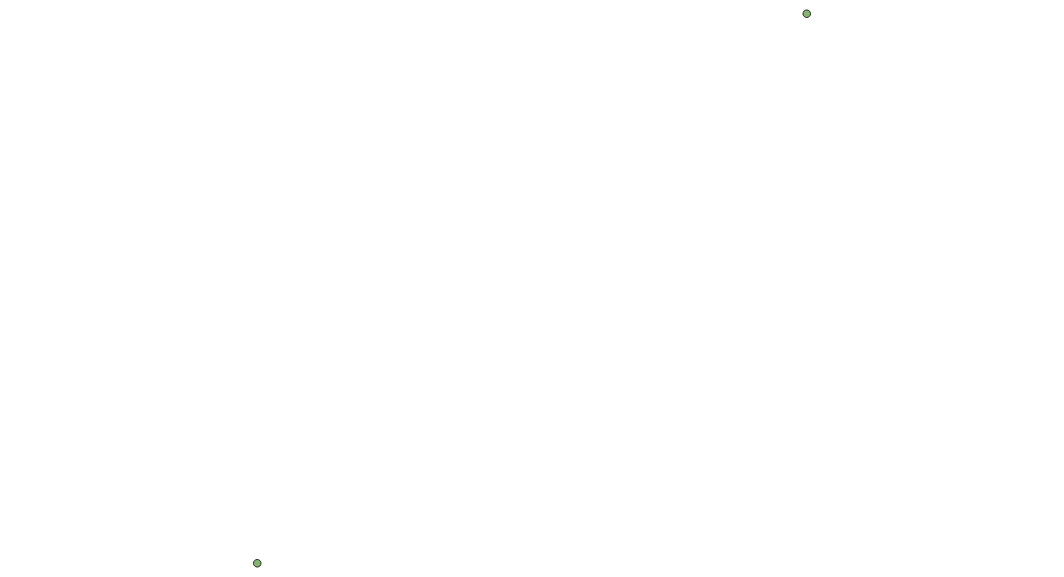
\includegraphics[width=6cm]{figures/Tugas2/1174077/no3.png}
		\centering
		\caption{Hasil No 3}
	\end{figure}
	\item Nomor 4
	\lstinputlisting{src/tugas2/1174077/no4.py}
	\begin{figure}[!htbp]
		
\includegraphics[width=6cm]{figures/Tugas2/1174077/no4.png}
		\centering
		\caption{Hasil No 4}
	\end{figure}
	\item Nomor 5
	\lstinputlisting{src/tugas2/1174077/no5.py}
	\begin{figure}[!htbp]
		
\includegraphics[width=6cm]{figures/Tugas2/1174077/no5.png}
		\centering
		\caption{Hasil No 5}
	\end{figure}
	\item Nomor 6
	\lstinputlisting{src/tugas2/1174077/no6.py}
	\begin{figure}[!htbp]
		
\includegraphics[width=6cm]{figures/Tugas2/1174077/no6.png}
		\centering
		\caption{Hasil No 6}
	\end{figure}
	\item Nomor 7
	\lstinputlisting{src/tugas2/1174077/no7.py}
	\begin{figure}[!htbp]
		
\includegraphics[width=6cm]{figures/Tugas2/1174077/no7.png}
		\centering
		\caption{Hasil No 7}
	\end{figure}
	\item Nomor 8
	\lstinputlisting{src/tugas2/1174077/no8.py}
	\begin{figure}[!htbp]
		
\includegraphics[width=6cm]{figures/Tugas2/1174077/no8.png}
		\centering
		\caption{Hasil No 8}
	\end{figure}
	\item Nomor 9
	\lstinputlisting{src/tugas2/1174077/no9.py}
	\begin{figure}[!htbp]
		
\includegraphics[width=6cm]{figures/Tugas2/1174077/no9.png}
		\centering
		\caption{Hasil No 9}
	\end{figure}
	\item Nomor 10
	\lstinputlisting{src/tugas2/1174077/no10.py}
	\begin{figure}[!htbp]
		
\includegraphics[width=6cm]{figures/Tugas2/1174077/no10.png}
		\centering
		\caption{Hasil No 10, NPM saya adalah 1174077, maka hasil modulus 8 dari NPM 1174077 adalah 5, jadi membuat bidang segitaga siku-siku dan angka kedua terakhir di NPM saya dalah 7 maka saya akan membuat 7 buah belah ketupat}
	\end{figure}
\end{enumerate}
\subsection{Link}
	https://youtu.be/a-UGqdoUFUo